\documentclass[12pt]{article}
\usepackage[left=1cm, right=1cm, top=2cm,bottom=1.5cm]{geometry} 

\usepackage[parfill]{parskip}
\usepackage[utf8]{inputenc}
\usepackage[T2A]{fontenc}
\usepackage[russian]{babel}
\usepackage{enumitem}
\usepackage[normalem]{ulem}
\usepackage{amsfonts, amsmath, amsthm, amssymb, mathtools}
\usepackage{tabularx}
\usepackage{hhline}

\usepackage{accents}
\usepackage{fancyhdr}
\pagestyle{fancy}
\renewcommand{\headrulewidth}{1.5pt}
\renewcommand{\footrulewidth}{1pt}

\usepackage{graphicx}
\usepackage[figurename=Рис.]{caption}
\usepackage{subcaption}
\usepackage{float}

%%Наименование папки откуда забирать изображения
\graphicspath{ {./images/} }

%%Изменение формата для ввода доказательства
\renewcommand{\proofname}{$\square$  \nopunct}
\renewcommand\qedsymbol{$\blacksquare$}

%%Изменение отступа на таблицах
\addto\captionsrussian{%
	\renewcommand{\proofname}{$\square$ \nopunct}%
}
%% Римские цифры
\newcommand{\RN}[1]{%
	\textup{\uppercase\expandafter{\romannumeral#1}}%
}

%% Для удобства записи
\newcommand{\MR}{\mathbb{R}}
\newcommand{\MC}{\mathbb{C}}
\newcommand{\MQ}{\mathbb{Q}}
\newcommand{\MN}{\mathbb{N}}
\newcommand{\MTB}{\mathbb{T}}
\newcommand{\MTI}{\mathbb{I}}
\newcommand{\MI}{\mathrm{I}}
\newcommand{\MJ}{\mathrm{J}}
\newcommand{\MH}{\mathrm{H}}
\newcommand{\MT}{\mathrm{T}}
\newcommand{\MU}{\mathcal{U}}
\newcommand{\MV}{\mathcal{V}}
\newcommand{\MB}{\mathcal{B}}
\newcommand{\MW}{\mathcal{W}}
\newcommand{\ML}{\mathcal{L}}
\newcommand{\VN}{\varnothing}
\newcommand{\VE}{\varepsilon}

\theoremstyle{definition}
\newtheorem{defn}{Опр:}
\newtheorem{rem}{Rm:}
\newtheorem{prop}{Утв.}
\newtheorem{exrc}{Упр.}
\newtheorem{lemma}{Лемма}
\newtheorem{theorem}{Теорема}
\newtheorem{corollary}{Следствие}

\newenvironment{cusdefn}[1]
{\renewcommand\thedefn{#1}\defn}
{\enddefn}

\DeclareRobustCommand{\divby}{%
	\mathrel{\text{\vbox{\baselineskip.65ex\lineskiplimit0pt\hbox{.}\hbox{.}\hbox{.}}}}%
}
%Короткий минус
\DeclareMathSymbol{\SMN}{\mathbin}{AMSa}{"39}
%Длинная шапка
\newcommand{\overbar}[1]{\mkern 1.5mu\overline{\mkern-1.5mu#1\mkern-1.5mu}\mkern 1.5mu}
%Функция знака
\DeclareMathOperator{\sgn}{sgn}

%Функция ранга
\DeclareMathOperator{\rk}{\text{rk}}

%Обозначение константы
\DeclareMathOperator{\const}{\text{const}}

\DeclareMathOperator*{\dsum}{\displaystyle\sum}
\newcommand{\ddsum}[2]{\displaystyle\sum\limits_{#1}^{#2}}

%Интеграл в большом формате
\DeclareMathOperator{\dint}{\displaystyle\int}
\newcommand{\ddint}[2]{\displaystyle\int\limits_{#1}^{#2}}
\newcommand{\ssum}[1]{\displaystyle \sum\limits_{n=1}^{\infty}{#1}_n}

\newcommand{\smallerrel}[1]{\mathrel{\mathpalette\smallerrelaux{#1}}}
\newcommand{\smallerrelaux}[2]{\raisebox{.1ex}{\scalebox{.75}{$#1#2$}}}

\newcommand{\smallin}{\smallerrel{\in}}
\newcommand{\smallnotin}{\smallerrel{\notin}}

\newcommand*{\medcap}{\mathbin{\scalebox{1.25}{\ensuremath{\cap}}}}%
\newcommand*{\medcup}{\mathbin{\scalebox{1.25}{\ensuremath{\cup}}}}%

\makeatletter
\newcommand{\vast}{\bBigg@{3.5}}
\newcommand{\Vast}{\bBigg@{5}}
\makeatother

%Промежуточное значение для sup\inf, поскольку они имеют разную высоту
\newcommand{\newsup}{\mathop{\smash{\mathrm{sup}}}}
\newcommand{\newinf}{\mathop{\mathrm{inf}\vphantom{\mathrm{sup}}}}

%Скалярное произведение
\DeclarePairedDelimiterX{\inner}[2]{\langle}{\rangle}{#1, #2}

%Подпись символов снизу
\newcommand{\ubar}[1]{\underaccent{\bar}{#1}}

%% Шапка для букв сверху
\newcommand{\wte}[1]{\widetilde{#1}}

%%Функция для обозначения равномерной сходимости по множеству
\newcommand{\uconv}[1]{\overset{#1}{\rightrightarrows}}
\newcommand{\uconvm}[2]{\overset{#1}{\underset{#2}{\rightrightarrows}}}


%%Функция для обозначения нижнего и верхнего интегралов
\def\upint{\mathchoice%
	{\mkern13mu\overline{\vphantom{\intop}\mkern7mu}\mkern-20mu}%
	{\mkern7mu\overline{\vphantom{\intop}\mkern7mu}\mkern-14mu}%
	{\mkern7mu\overline{\vphantom{\intop}\mkern7mu}\mkern-14mu}%
	{\mkern7mu\overline{\vphantom{\intop}\mkern7mu}\mkern-14mu}%
	\int}
\def\lowint{\mkern3mu\underline{\vphantom{\intop}\mkern7mu}\mkern-10mu\int}


\begin{document}
\lhead{Математический анализ - \RN{3}}
\chead{Шапошников С.В.}
\rhead{Лекция - 22}
\section*{Собственный интеграл с параметром}
Пусть $f(x,y) \colon [a,b]\times [c,d] \to \MR (\MC)$. Предположим, что $\forall y$ функция $x \mapsto f(x,y)$ интегрируема на $[a,b]$ по Риману. Пусть также есть какие-то функции $\alpha,\beta \colon [c,d] \to [a,b]$. 

\begin{defn}
	\uwave{Собственным интегралом с параметром} мы будем называть функцию на $[c,d]$ вида:
	$$
		F(y) = \ddint{\alpha(y)}{\beta(y)}f(x,y)dx
	$$	
\end{defn}

Возникает несколько вопросов про эту функцию: 
\begin{enumerate}[label=\arabic*)]
	\item \textbf{Непрерывность};
	\item \textbf{Дифференцируемость};
	\item \textbf{Интегрируемость};
\end{enumerate}
\begin{rem}
	Разобравшись с этими вопросами, мы перенесем их на несобственные интегралы и там \\ понадобится равномерная сходимость.
\end{rem}
\subsection*{Непрерывность собственного интеграла с параметром}
\begin{theorem}
	Пусть $f \in C([a,b]\times[c,d])$ - непрерывна на квадрате и $\alpha,\beta \in C([c,d])$ - непрерывны на отрезке. Тогда  функция: 
	$$
		F(y) = \ddint{\alpha(y)}{\beta(y)}f(x,y)dx
	$$
	непрерывна на отрезке $[c,d]$.
\end{theorem}
\begin{proof}
	Введем вспомогательную функцию:
	$$
		\Phi(u,y) = \ddint{a}{u}f(x,y)dx,\, y \in [c,d], \, u \in [a,b]
	$$
	тогда: 
	$$
		F(y) = \ddint{\alpha(y)}{\beta(y)}f(x,y)dx = \ddint{\alpha(y)}{u}f(x,y)dx + \ddint{u}{\beta(y)}f(x,y)dx  = \Phi(\beta(y), y) - \Phi(\alpha(y),y)
	$$ 
	Достаточно проверить, что функция $\Phi(u,y)$ - непрерывна на $[a,b]\times[c,d]$ по совокупности переменных. \\ Пусть $(u_0, y_0) \in [a,b]\times [c,d]$, следовательно:
	$$
		\left|\Phi(u,y) - \Phi(u_0,y_0)\right| \leq  \left|\Phi(u,y) - \Phi(u,y_0)\right| + \left|\Phi(u,y_0) - \Phi(u_0,y_0)\right|
	$$
	Рассмотрим второе слагаемое в неравенстве:
	$$
		\left|\Phi(u,y_0) - \Phi(u_0,y_0)\right| = \left| \ddint{u_0}{u}f(x,y_0)dx \right|
	$$
	Поскольку $f(x,y)$ - непрерывна на $[a,b]\times [c,d]$, значит она ограничена на нём. Тогда:
	$$
		\exists\, M > 0 \colon \forall (x,y) \in [a,b]\times [c,d], \, |f(x,y)| \leq M \Rightarrow \left| \ddint{u_0}{u}f(x,y_0)dx \right| \leq \ddint{u_0}{u}|f(x,y_0)|dx \leq M|u - u_0|
	$$  
	Таким образом: $M|u - u_0| \xrightarrow[u \to u_0]{}0$. Рассмотрим первое слагаемое в неравенстве:
	$$
		\left|\Phi(u,y) - \Phi(u,y_0)\right| \leq \ddint{a}{u}|f(x,y) - f(x,y_0)|dx \leq \ddint{a}{b}|f(x,y) - f(x,y_0)|dx
	$$
	Поскольку $f(x,y)$ - непрерывна на прямоугольнике $\Rightarrow f(x,y) \uconvm{[a,b]}{y \to y_0} f(x,y_0)$ по теореме Кантора (см. пример в лекции $20$ этого семестра), тогда:
	$$
		\lim\limits_{y \to y_0}\ddint{a}{b}|f(x,y) - f(x,y_0)|dx = \ddint{a}{b}\lim\limits_{y \to y_0} |f(x,y) - f(x,y_0)|dx = 0
	$$
	Следовательно, $\lim\limits_{(u,y) \to (u_0, y_0)}\Phi(u,y) = \Phi(u_0,y_0) \Rightarrow \Phi(u,y)$ - по определению непрерывна по совокупности переменных. Исходная функция $F(y)$ - композиция непрерывных функций $\Rightarrow$ непрерывна.
\end{proof}
\begin{proof}(\textbf{второе доказательство})
	Можем доказать по-другому, используя ту же функцию $\Phi(u,y)$. Всё также покажем, что эта она непрерывна по совокупности переменных. Если $y$ - фиксированный, то:
	$$
		u \mapsto \ddint{a}{u}f(x,y)dx
	$$ 
	непрерывная функция (см. например, семестр $2$, лекция $26$, утверждение $2$ про Липшецевость), поскольку $f(x,y)$ - непрерывна (хотя достаточно и интегрируемости). Зафиксируем переменную $u$, тогда рассмотрим функцию:
	$$	
		y \mapsto \ddint{a}{u}f(x,y)dx
	$$
	она также будет непрерывна в силу рассуждений, аналогичных предыдущему доказательству:
	$$
		f(x,y) \in C([a,b]\times[c,d]) \Rightarrow f(x,y) \uconvm{[a,b]}{y \to y_0} f(x,y_0) \Rightarrow \lim\limits_{y \to y_0}\ddint{a}{u}f(x,y)dx = \ddint{a}{u}f(x,y_0)dx
	$$
	Для получения непрерывности $\Phi(u,y)$ по совокупности переменных нам нужно, чтобы она была равномерно непрерывной хотя бы по одной переменной относительно другой (см. семестр $2$, лекция $10$). Аналогично предыдущему доказательству:
	$$
		f(x,y) \in C([a,b]\times[c,d]) \Rightarrow \exists\, M > 0 \colon \forall (x,y) \in [a,b]\times [c,d], \, |f(x,y)| \leq M \Rightarrow
	$$
	$$
		\left|\Phi(u,y) - \Phi(v,y)\right| = \left| \ddint{v}{u}f(x,y)dx \right| \leq \ddint{v}{u}|f(x,y)|dx \leq M|u - v| \xrightarrow[v \to u]{}0 \Rightarrow \Phi(u,y) \uconvm{[c,d]}{u \to u_0} \Phi(u_0,y) 
	$$
	Таким образом, мы получили $\Phi(u,y)$ - непрерывная функция по совокупности переменных.
\end{proof}
\subsection*{Дифференцируемость собственного интеграла с параметром}
\begin{theorem}
	Пусть $f\colon [a,b]\times[c,d]\to \MR$ - непрерывна, $\forall x$ функция $y \mapsto f(x,y)$ - непрерывно дифференцируема на $[c,d]$ или, что то же самое, $f_y^\prime(x,y)$ - непрерывна на $[a,b] \times [c,d]$ и функции $\alpha, \beta$ - непрерывно дифференцируемы на $[c,d]$. Тогда функция: 
	$$
		F(y) = \ddint{\alpha(y)}{\beta(y)}f(x,y)dx
	$$
	будет непрерывно дифференцируема и справедливо равенство:
	$$
		F^\prime(y) = \beta^\prime(y) {\cdot}f(\beta(y),y) - \alpha^\prime(y){\cdot}f(\alpha(y),y) + \ddint{\alpha(y)}{\beta(y)}f_y^\prime(x,y)dx
	$$
\end{theorem}
\begin{rem}
	В комплексном случае $f\colon [a,b]\times[c,d]\to \MC$, $f(x,y) = u(x,y) + i v(x,y), \, f_y^\prime = u_y^\prime + i v_y^\prime$. Соответственно, исследуемая функция будет иметь вид:
	$$
		F(y) = \ddint{\alpha(y)}{\beta(y)}u(x,y)dx + i \ddint{\alpha(y)}{\beta(y)}v(x,y)dx
	$$
	И мы применяем теорему к каждому из этих интегралов по отдельности.
\end{rem}
\begin{rem}
	Заметим также, что формула дифференцирования немного не интуитивна и бывает полезно рассмотреть случай, когда $f(x,y) = f(x)$, тогда будет получаться:
	$$
		F(y) = \ddint{\alpha(y)}{\beta(y)}f(x)dx \Rightarrow F^\prime(y) = \beta^\prime(y) {\cdot}f(\beta(y)) - \alpha^\prime(y){\cdot}f(\alpha(y))
	$$
\end{rem}
\begin{proof}
	Воспользуемся вспомогательной функцией $\Phi(u,y)$:
	$$
		\Phi(u,y) = \ddint{a}{u}f(x,y)dx \Rightarrow F(y) = \Phi(\beta(y),y) - \Phi(\alpha(y),y)
	$$
	Если уже знаем, что $\Phi(u,y)$ - непрерывно дифференцируема, то $F^\prime(y)$ будет равна:
	$$
		F^\prime(y) = \dfrac{\partial \Phi}{\partial u}(\beta(y),y){\cdot}\beta^\prime(y) + \dfrac{\partial \Phi}{\partial y}(\beta(y),y)  - \dfrac{\partial \Phi}{\partial u}(\alpha(y),y){\cdot}\alpha^\prime(y) - \dfrac{\partial \Phi}{\partial y}(\alpha(y),y)
	$$
	Поскольку $\Phi(u,y)$ это интеграл с переменным верхним пределом, то его производные будет равны:
	$$
		\dfrac{\partial \Phi}{\partial u}(u,y) = f(u,y), \, \dfrac{\partial \Phi}{\partial y}(u,y) = \dfrac{\partial}{\partial y} \left(\ddint{a}{u}f(x,y)dx\right)
	$$
	Если интеграл и дифференцирование можно переставлять местами, то $F^\prime(y)$ приобретет вид:
	$$
		F^\prime(y) = f(\beta(y),y){\cdot}\beta^\prime(y) + \ddint{a}{\beta(y)}\dfrac{\partial f}{\partial y}(x,y)dx - f(\alpha(y),y){\cdot}\alpha^\prime(y) - \ddint{a}{\alpha(y)}\dfrac{\partial f}{\partial y}(x,y)dx =
	$$
	$$
		=  f(\beta(y),y){\cdot}\beta^\prime(y) - f(\alpha(y),y){\cdot}\alpha^\prime(y) + \ddint{\alpha(y)}{\beta(y)}\dfrac{\partial f}{\partial y}(x,y)dx
	$$
	И соответственно мы получаем требуемое. Значит нам нужно показать дифференцируемость $\Phi(u,y)$ и возможность переставить интеграл и производную местами. По определению дифференцирования интеграла с переменным верхним пределом от непрерывной функции:
	$$
		\dfrac{\partial \Phi}{\partial u}(u,y) = f(u,y) \in C([a,b]\times [c,d])
	$$
	Функция $f(x,y)$ - непрерывна по условию, значит производная по первому аргументу - непрерывна (поскольку равна непрерывной функции $f(u,y)$). Если мы проверим равенство:
	$$
		\dfrac{\partial \Phi}{\partial y}(u,y) =  \ddint{a}{u}\dfrac{\partial f}{\partial y}(x,y)dx
	$$
	где $f_y^\prime(x,y)$ - непрерывная по условию $\Rightarrow$ интеграл с переменным верхним пределом от непрерывной функции будет по совокупности переменных непрерывным (см. предыдущую теорему). Если частные производные оказались непрерывными, то сама функция - дифференцируема (см. достаточное условие, семестр $2$, лекция $13$). И даже больше, она будет непрерывно дифференцируема, поскольку частные первые производные - непрерывные (или ещё рассуждая так: композиция непр. дифф. функций - непрерывно дифференцируема). Таким образом, нам необходимо доказать последнее равенство:
	$$
		\dfrac{\partial \Phi}{\partial y}(u,y) =	\lim\limits_{y \to y_0} \dfrac{\Phi(u,y) - \Phi(u,y_0)}{y - y_0} = \lim\limits_{y \to y_0}\ddint{a}{u}\dfrac{f(x,y) - f(x,y_0)}{y - y_0}dx = \ddint{a}{u}\dfrac{\partial f}{\partial y}(x,y_0)dx
	$$
	где последнее верно в силу теоремы Арцела, поскольку $f_y^\prime(x,y)$ - непрерывна $\Rightarrow$ интегрируема, разница непрерывных функций - непрерывная функция $\Rightarrow$ интегрируема и есть оценка:
	$$
		\left| \dfrac{f(x,y) - f(x,y_0)}{y - y_0} \right| = \left| \dfrac{\partial f}{\partial y}(x,c) \right| \leq C
	$$
	где равенство верно по теореме Лагранжа, но $f_y^\prime(x,y)$ непрерывна на прямоугольнике и поэтому вся ограничена какой-то константой $C > 0$.
	
	Можно это же показать через равномерную сходимость:
	$$
		\sup\limits_{x \in [a,b]}\left| \dfrac{f(x,y) - f(x,y_0)}{y - y_0} - \dfrac{\partial f}{\partial y}(x,y) \right| = \sup\limits_{x \in [a,b]}\left| \dfrac{\partial f}{\partial y}(x,c) - \dfrac{\partial f}{\partial y}(x,y) \right|, \, \lim\limits_{y\to y_0}c(y) = y_0
	$$
	где равенство верно в силу теоремы Лагранжа и точка $c$ лежит между $y$ и $y_0$. Поскольку функция \\ $f_y^\prime(x,y) \in C([a,b]\times [c,d])$, то она равномерно непрерывна на этом прямоугольнике. Тогда:
	$$
		\dfrac{\partial f}{\partial y}(x,y) \uconvm{[a,b]}{y\to y_0} \dfrac{\partial f}{\partial y}(x,y_0) \Rightarrow
		\sup\limits_{x \in [a,b]}\left| \dfrac{\partial f}{\partial y}(x,c) - \dfrac{\partial f}{\partial y}(x,y) \right| \xrightarrow[y \to y_0]{}0
	$$
	Следовательно, мы можем переставить интеграл и предел местами (по теореме о перестановке предела и интеграла для несобственных интегралов).
\end{proof}
\subsection*{Интегрируемость собственного интеграла с параметром}
\begin{theorem}
	Пусть $f \in C([a,b]\times [c,d])$ и $F(y) = \ddint{a}{b}f(x,y)dx$. Тогда $F(y)$ интегрируема на $[c,d]$, \\ функция $x \mapsto \ddint{c}{d}f(x,y)dy$ интегрируема на $[a,b]$ и верно равенство:
	$$
		\ddint{c}{d}F(y)dy = \ddint{c}{d}\left(\ddint{a}{b}f(x,y)dx\right)dy = \ddint{a}{b}\left(\ddint{c}{d}f(x,y)dy\right)dx
	$$
\end{theorem}
\begin{proof}
	Поскольку $f(x,y)$ - непрерывна по $y \Rightarrow F(y)$ тоже непрерывна по теореме $1 \Rightarrow$ функция $F(y)$ интегрируема по  $y$. Аналогично для функции $x \mapsto \ddint{c}{d}f(x,y)dy$: она также будет непрерывной $\Rightarrow$ интегрируемой по $x$. Обоснуем перестановку интегралов местами, рассмотрим разность:
	$$
		 \ddint{c}{d}\left(\ddint{a}{b}f(x,y)dx\right)dy - \ddint{a}{b}\left(\ddint{c}{d}f(x,y)dy\right)dx
	$$
	Заменим $b$ на $t$, где $t \in [a,b]$ и рассмотрим функцию $\psi(t)$:
	$$
		\forall t \in [a,b], \, \psi(t) = \ddint{c}{d}\left(\ddint{a}{t}f(x,y)dx\right)dy - \ddint{a}{t}\left(\ddint{c}{d}f(x,y)dy\right)dx \Rightarrow \psi(a) \overset{?}{=} 0
	$$
	Продифференцируем $\psi(x)$: поскольку $f(x,y)$ - непрерывна, то интеграл с переменным верхним пределом от неё непрерывно дифференцируем по $t$:
	$$
		f(x,y) \in C([a,b]\times [c,d]) \Rightarrow \dfrac{\partial}{\partial t}\left(\ddint{a}{t}f(x,y)dx\right) = f(t,y) \in C([a,b]\times [c,d])
	$$
	Следовательно, можно применить вторую теорему к первому слагаемому $\psi(t)$: 
	$$
		\dfrac{d}{d t}\left(\ddint{c}{d}\left(\ddint{a}{t}f(x,y)dx\right)dy\right) = \ddint{c}{d}\left(\dfrac{\partial}{\partial t}\left(\ddint{a}{t}f(x,y)dx\right)\right)dy = \ddint{c}{d}f(t,y)dy
	$$
	Второй интеграл дифференцируется, как интеграл с переменным верхним пределом от непрерывной функции. Тогда:
	$$
		\psi^\prime(t) = \ddint{c}{d}f(t,y)dy - \ddint{c}{d}f(t,y)dy = 0 \Rightarrow \psi(t) \equiv 0 \Rightarrow \psi(b) = 0
	$$
	Поскольку в точке $a$ функция $\psi(t)$ равна $0$, и её производная $\psi^\prime(t) \equiv 0$.
\end{proof}

\begin{rem}
	Отметим, что в следующем семестре мы будем рассматривать гораздо более общую теорему Фубини, поэтому общность в данном случае нас пока не будет сильно интересовать.
\end{rem}

Фактически, нами доказано следующее равенство для непрерывной функции $f(x,y)$:
$$
	\ddint{c}{d}\left(\ddint{a}{b}f(x,y)dx\right)dy = \ddint{a}{b}\left(\ddint{c}{d}f(x,y)dy\right)dx
$$
Рассмотрим прямоугольник $[a,b]\times[c,d]$ и сделаем его разбиение точками $\{x_k\}$ и $\{y_m\}$ сторон $[a,b]$ и $[c,d]$ соответственно:
\begin{figure}[H]
	\centering
	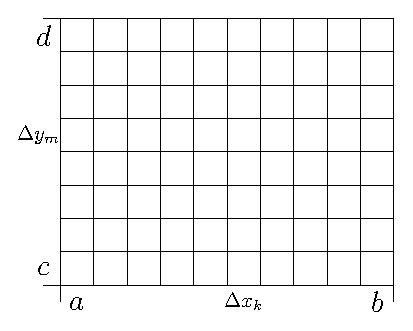
\includegraphics[width=0.3\textwidth]{MA3L22_1.eps}
	\label{MA3L22_1}
	\caption{Разбиение прямоугольника $[a,b]\times [c,d]$.}
	\label{fig:прямоугольник с повторными интегралами}
\end{figure}
Мы знаем, что когда масштаб разбиения стремится к нулю, то $\ddint{a}{b}f(x,y)dx \approx \ddsum{k = 1}{N}f(x_k, y){\cdot}|\Delta x_k|$, интеграл приближается своей Римановой суммой. Эвристически отсюда можно сделать вывод:
$$
	\ddint{c}{d}\left(\ddint{a}{b}f(x,y)dx\right)dy \approx \ddsum{m = 1}{M}\ddsum{k = 1}{N}f(x_k, y_m){\cdot}|\Delta x_k| {\cdot}|\Delta y_m|, \, \ddint{a}{b}f(x,y_m)dx \approx \ddsum{k = 1}{N}f(x_k, y_m){\cdot}|\Delta x_k|
$$
Поскольку сумму можно считать в любом порядке, то мы можем поменять порядок и получим:
$$
	\ddsum{m = 1}{M}\ddsum{k = 1}{N}f(x_k, y_m){\cdot}|\Delta x_k{\cdot}|\Delta y_m| = \ddsum{k = 1}{N}\ddsum{m = 1}{M}f(x_k, y_m) {\cdot}|\Delta y_m|{\cdot}|\Delta x_k|, \, \ddsum{m = 1}{M}f(x_k, y_m) {\cdot}|\Delta y_m| \approx \ddint{c}{d}f(x_k,y)dy \Rightarrow
$$
$$
	\Rightarrow \ddsum{k = 1}{N}\ddsum{m = 1}{M}f(x_k, y_m){\cdot} |\Delta y_m|{\cdot}|\Delta x_k| \approx \ddint{a}{b}\left(\ddint{c}{d}f(x,y)dy\right)dx
$$
Таким способом, мы получили естественную логику на основе которой возникает равенство в теореме выше. Попробуем его доказать формально.
\begin{proof}
	Заметим, что поскольку $f(x,y) \in C([a,b]\times [c,d])$, то $f(x,y)$ - равномерно непрерывна на этом прямоугольнике. Из примера в лекции $20$:
	$$
		\forall \VE > 0, \, \exists \, \delta_1 > 0 \colon \forall x \in [a,b], \, |x - x_0| < \delta_1 \Rightarrow \sup\limits_{y \in [c,d]}|f(x,y) - f(x_0,y)| < \VE
	$$
	Также из теоремы $1$ мы знаем, что $F(y) = \ddint{a}{b}f(x,y)dx$ - непрерывная функция $\Rightarrow$ интегрируема. По определению интегрируемости по Риману:
	$$
		\forall \VE > 0,\, \exists \, \delta_2 > 0 \colon \forall (\MTB_y, \eta), \, \lambda(\MTB_y) < \delta_2 \Rightarrow \left|\ddsum{m = 1}{M}F(\eta_m){\cdot}|\Delta y_m| - \ddint{c}{d}F(y)dy \right| < \VE
	$$
	Рассмотрим следующую разность и прибавим-вычтем сумму $\ddsum{m = 1}{M}F(\eta_m){\cdot}|\Delta y_m|$:
	$$
		\left|\ddsum{m = 1}{M}\ddsum{k = 1}{N}f(\xi_k,\eta_m){\cdot}|\Delta x_k|{\cdot}|\Delta y_m| - \ddint{c}{d}\left(\ddint{a}{b}f(x,y)dx\right)dy \right| = 
	$$
	$$
		= \left|\ddsum{m = 1}{M}\left(\ddsum{k = 1}{N}f(\xi_k,\eta_m){\cdot}|\Delta x_k| - F(\eta_m)\right){\cdot}|\Delta y_m|  + \ddsum{m = 1}{M}F(\eta_m){\cdot}|\Delta y_m| -  \ddint{c}{d}F(y)dy \right| \leq
	$$
	$$
		\leq \ddsum{m = 1}{M}\left|\ddsum{k = 1}{N}f(\xi_k,\eta_m){\cdot}|\Delta x_k| - F(\eta_m)\right|{\cdot}|\Delta y_m| + \left|\ddsum{m = 1}{M}F(\eta_m){\cdot}|\Delta y_m| -  \ddint{c}{d}F(y)dy \right|
	$$
	Мы знаем как оценить правую часть $\Rightarrow$ необходимо понять как можно оценить левую. По определению интегрируемости по Риману при фиксированном $y \in [c,d]$:
	$$
		\forall \VE > 0,\, \exists \, \delta_3 > 0 \colon \forall (\MTB_x, \xi), \, \lambda(\MTB_x) < \delta_3 \Rightarrow \left|\ddsum{k = 1}{N}f(\xi_k,y){\cdot}|\Delta x_k| - \ddint{a}{b}f(x,y)dx \right| < \VE
	$$
	$$
		\sup\limits_{y \in [c,d]}\left|\ddsum{k = 1}{N}f(\xi_k,y){\cdot}|\Delta x_k| - \ddint{a}{b}f(x,y)dx \right| \leq \ddsum{k = 1}{N} \left(\;\ddint{x_{k-1}}{x_k}\sup\limits_{y \in [c,d]}\left|f(\xi_k,y) - f(x,y)\right|dx\right)
	$$
	Пусть $\bar{\delta} = \min\{\delta_1,\delta_3\}$, тогда если $\lambda(\MTB_x) < \bar{\delta}$, то $\max\limits_{k}|\Delta x_k| < \bar{\delta} \Rightarrow \forall x \in [x_{k-1}, x_k], \, |x - \xi_k| < \delta_1$ и по равномерной непрерывности мы получим, что $\sup\limits_{y \in [c,d]}|f(x,y) - f(\xi_k,y)|< \VE$. Тогда:
	$$
		\sup\limits_{y \in [c,d]}\left|\ddsum{k = 1}{N}f(\xi_k,y){\cdot}|\Delta x_k| - \ddint{a}{b}f(x,y)dx \right| \leq \VE {\cdot}\ddsum{k = 1}{N}|\Delta x_k| = \VE (b-a) \Rightarrow
	$$
	$$
		\Rightarrow \ddsum{m = 1}{M}\left|\ddsum{k = 1}{N}f(\xi_k,\eta_m){\cdot}|\Delta x_k| - F(\eta_m)\right|{\cdot}|\Delta y_m| \leq \VE(b-a)\ddsum{k = 1}{M}|\Delta y_m| = \VE (b-a)(d - c)
	$$
	Таким образом, если мы выбираем $\hat{\delta} = \min\{\bar{\delta}, \delta_3\}$ маленькой, то мы получим следующий результат:
	$$
		\forall \VE > 0, \, \exists \, \hat{\delta} > 0 \colon \max\{\lambda(\MTB_x), \lambda(\MTB_y)\} < \hat{\delta} \Rightarrow \left|\ddsum{m = 1}{M}\ddsum{k = 1}{N}f(\xi_k,\eta_m){\cdot}|\Delta x_k|{\cdot}|\Delta y_m| - \ddint{c}{d}\left(\ddint{a}{b}f(x,y)dx\right)dy \right| < \VE
	$$
	для любого подходящего разбиения. Аналогичным образом получается:
	$$
		\forall \VE > 0, \, \exists \, \delta > 0 \colon \max\{\lambda(\MTB_x), \lambda(\MTB_y)\} < \delta \Rightarrow \left|\ddsum{k = 1}{N}\ddsum{m = 1}{M}f(\xi_k,\eta_m){\cdot}|\Delta y_m|{\cdot}|\Delta x_k| - \ddint{a}{b}\left(\ddint{c}{d}f(x,y)dy\right)dx \right| < \VE
	$$
	Поскольку сумма при перестановке слагаемых не изменяется, то мы получаем требуемое:
	$$
		\lim\limits_{(\lambda(\MTB_x),\lambda(\MTB_y)) \to (0,0)}\ddsum{m = 1}{M}\ddsum{k = 1}{N}f(\xi_k,\eta_m){\cdot}|\Delta x_k|{\cdot}|\Delta y_m| = \ddint{c}{d}\left(\ddint{a}{b}f(x,y)dx\right)dy = \ddint{a}{b}\left(\ddint{c}{d}f(x,y)dy\right)dx
	$$
\end{proof}

Также заметим, что теорему о дифференцируемости по параметру можно вывести из утверждения про интегрируемость. То есть, до этого мы вывели теорему об интегрируемости из теоремы про дифференцируемость, а теперь можем сделать всё наоборот. Основным моментом в теореме про дифференцируемость было следующее:
$$
	\dfrac{\partial \Phi}{\partial y}(u,y) = \dfrac{d}{dy}\left(\ddint{a}{u}f(x,y)dx \right)=  \ddint{a}{u}\dfrac{\partial f}{\partial y}(x,y)dx
$$
Проинтегрируем левую часть этого равенства ещё раз по второму аргументу от $c$ до $y$:
$$
	\ddint{c}{y}\left(\dfrac{d}{dt}\ddint{a}{u}f(x,t)dx\right) dt = \ddint{a}{u}f(x,y) dx - \ddint{a}{u}f(x,c)dx
$$
где мы применили формулу Ньютона-Лейбница. И проинтегрируем правую часть:
$$
	\ddint{c}{y}\left(\ddint{a}{u}\dfrac{\partial f}{\partial t}(x,t)dx\right)dt = \ddint{a}{u}\left(\ddint{c}{y}\dfrac{\partial f}{\partial t}(x,t) dt\right)dx = \ddint{a}{u}(f(x,y) - f(x,c))dx = \ddint{a}{u}f(x,y) dx - \ddint{a}{u}f(x,c)dx
$$
где во втором равенстве мы применили теорему об интегрируемости интеграла с параметром. Видим, что значения левой и правой части исходного равенства при интегрировании совпали. Теперь можно проделать доказательство равенства задом наперед:
$$
	\ddint{a}{u}f(x,y) dx - \ddint{a}{u}f(x,c)dx = \ddint{a}{u}(f(x,y) - f(x,c))dx = \ddint{a}{u}\left(\ddint{c}{y}\dfrac{\partial f}{\partial t}(x,t) dt\right)dx
	= \ddint{c}{y}\left(\ddint{a}{u}\dfrac{\partial f}{\partial t}(x,t)dx\right)dt
$$
где последний интгерал - дифференцируем как интеграл с переменным верхним пределом, тогда дифференцируема левая часть равенства и будет верно:
$$ 
	\dfrac{d}{dy}\ddint{a}{u}f(x,y)dx - 0 = \dfrac{d}{dy}\ddint{a}{u}f(x,y)dx=  \ddint{a}{u}\dfrac{\partial f}{\partial y}(x,y)dx
$$
\newpage
\begin{exrc}
	Используя равенство $\ddint{a}{b}f(x,y)dx = \lim\limits_{\lambda(\MTB) \to 0}\ddsum{k = 1}{N}f(\xi_k,y){\cdot}|\Delta x_k|$ доказать теорему о дифференцируемости по параметру собственного интеграла с параметром.
\end{exrc}
\begin{proof}
	Распишем производную по определению и воспользуемся линейностью интеграла:
	$$
		\dfrac{d}{dy}\left(\ddint{a}{b}f(x,y)dx\right) = \lim\limits_{\Delta y \to 0}\dfrac{\ddint{a}{b}f(x, y + \Delta y)dx - \ddint{a}{b}f(x,y)dx}{\Delta y} = \lim\limits_{\Delta y \to 0}\ddint{a}{b}\dfrac{f(x, y + \Delta y) - f(x,y)}{\Delta y} dx =
	$$
	$$
		= \lim\limits_{\Delta y \to 0}\lim\limits_{\lambda(\MTB)\to 0}\ddsum{k = 1}{N}\dfrac{f(\xi_k, y + \Delta y) - f(\xi_k, y)}{\Delta y}{\cdot}|\Delta x_k| = \lim\limits_{\Delta y \to 0}\lim\limits_{\lambda(\MTB)\to 0}\psi\left(\lambda(\MTB) , \Delta y\right)
	$$
	Рассмотрим предел функции $\psi(\lambda(\MTB) , \Delta y)$ при $\Delta y \to 0$:
	$$
		\lim\limits_{\Delta y \to 0}\psi(\lambda(\MTB) , \Delta y) = \lim\limits_{\Delta y \to 0}\ddsum{k = 1}{N}\dfrac{f(\xi_k, y + \Delta y) - f(\xi_k, y)}{\Delta y}{\cdot}|\Delta x_k| = 
	$$
	$$
		= \ddsum{k = 1}{N}\left(\lim\limits_{\Delta y \to 0}\dfrac{f(\xi_k, y + \Delta y) - f(\xi_k, y)}{\Delta y} \right){\cdot}|\Delta x_k| = \ddsum{k = 1}{N}\dfrac{\partial f}{\partial y}(\xi_k, y){\cdot}|\Delta x_k|
	$$
	Если мы покажем, что этот предел равномерный, то сможем воспользоватсья теоремой о перестановке пределов и получить требуемое. Рассмотрим разность:
	$$
		\left|\ddsum{k = 1}{N}\dfrac{f(\xi_k, y+\Delta y) - f(\xi_k, y)}{\Delta y}{\cdot}|\Delta x_k| - \ddsum{k = 1}{N}\dfrac{\partial f}{\partial y}(\xi_k, y){\cdot}|\Delta x_k|\right| \leq 
	$$
	$$
		\leq \ddsum{k = 1}{N}\left|\dfrac{f(\xi_k, y+\Delta y) - f(\xi_k, y)}{\Delta y} - \dfrac{\partial f}{\partial y}(\xi_k, y)\right|{\cdot}|\Delta x_k| = \ddsum{k = 1}{N}\left| \dfrac{\partial f}{\partial y}(\xi_k, c_0) - \dfrac{\partial f}{\partial y}(\xi_k, y)  \right|{\cdot}|\Delta x_k|, \, c_0 \in (y, y + \Delta y)
	$$
	где мы воспользовались теоремой Лагранжа, в силу непрерывной дифференцируемости $f(x,y)$ по $y$. Поскольку $f(x,y)$ - непрерывно дифференцируема по $y$, то $f_y^\prime(x,y)$ - непрерывна на $[c,d] \Rightarrow$ равномерно непрерывна на отрезке (по теореме Кантора). Тогда по определению:
	$$
		\forall \VE > 0, \, \exists \, \delta > 0 \colon \forall y,y_0 \in [c,d], \, |y - y_0| < \delta \Rightarrow \sup\limits_{x \in [a,b]}\left|\dfrac{\partial f}{\partial y}(x, y) - \dfrac{\partial f}{\partial y}(x, y_0) \right| < \VE
	$$
	Тогда, зафиксировав $\VE > 0$, найдем $\delta > 0$ такой, что $|\Delta y | < \delta \Rightarrow \forall y \in [c,d], \, |y - c_0| < \delta$, тогда:
	$$
		\forall \xi_k, \, \left| \dfrac{\partial f}{\partial y}(\xi_k, c_0) - \dfrac{\partial f}{\partial y}(\xi_k, y)  \right| \leq \sup\limits_{x \in [a,b]}\left|\dfrac{\partial f}{\partial y}(x, y) - \dfrac{\partial f}{\partial y}(x, c_0) \right| < \VE \Rightarrow
	$$
	$$
		\Rightarrow \forall (\MTB, \xi),\, \left|\ddsum{k = 1}{N}\dfrac{f(\xi_k, y+\Delta y) - f(\xi_k, y)}{\Delta y}{\cdot}|\Delta x_k| - \ddsum{k = 1}{N}\dfrac{\partial f}{\partial y}(\xi_k, y){\cdot}|\Delta x_k|\right| \leq \ddsum{k = 1}{N}\VE{\cdot}|\Delta x_k| = \VE (b- a) \Rightarrow
	$$
	$$
		\psi(\lambda(\MTB), \Delta y) \uconvm{(\MTB,\xi)}{\Delta y \to 0} \ddsum{k = 1}{N}\dfrac{\partial f}{\partial y}(\xi_k, y){\cdot}|\Delta x_k| \Rightarrow \lim\limits_{\Delta y \to 0}\lim\limits_{\lambda(\MTB)\to 0}\psi\left(\lambda(\MTB),\Delta y\right) = \lim\limits_{\lambda(\MTB)\to 0}\lim\limits_{\Delta y \to 0}\psi\left(\lambda(\MTB),\Delta y\right) 
	$$
\end{proof}
\begin{exrc}
	Пусть $f \in C([a,b]\times[a,b])$, доказать равенство:
	$$
		\ddint{a}{b}\left(\ddint{a}{y}f(x,y)dx\right) dy = \ddint{a}{b}\left(\ddint{x}{b}f(x,y)dy\right) dx
	$$
\end{exrc}
\begin{rem}
	Возникает вопрос, откуда появляются такие равенства? Рассмотрим квадрат $[a,b]\times [a,b]$ и возьмем его диагональ $y = x$. Если интегралы заменить суммами, то в равенстве будет написано: надо суммировать по $x$, при фиксированном $y$, от $a$ до $y$. То есть фиксируем $y$ (например, $y_k$) и суммируем по $x$ только до диагонали (а не по всей строчке):
	\begin{figure}[H]
		\centering
		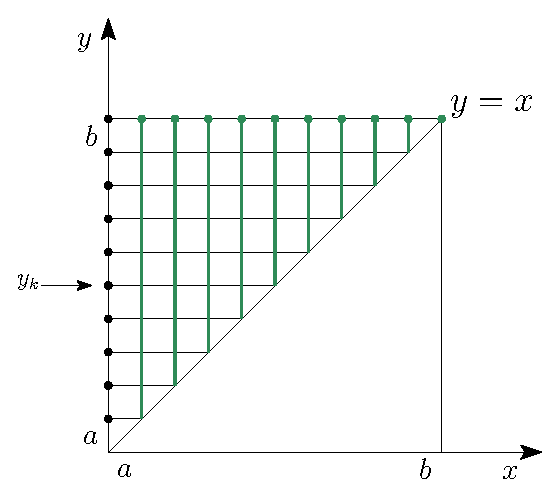
\includegraphics[width=0.35\textwidth]{MA3L22_2.eps}
		\label{MA3L22_2}
		\caption{Мотивация для равенства повторных интегралов с переменными пределами.}
		\label{fig:равенство повторных интегралов}
	\end{figure}
	И дальше суммируем по $y \Rightarrow$ нашли сумму всех элементов таблицы в верхнем треугольнике. С другой стороны, при фиксированном $x$ мы можем суммировать по столбцам от диагонали (от $x$ до $b$), а затем сложить результат. Получим тот же результат: сумму всех элементов в верхнем треугольнике.
\end{rem}

\begin{proof}
	Рассмотрим следующую функцию:
	$$
		\psi(t) = \ddint{a}{t}\left(\ddint{a}{y}f(x,y)dx\right)dy - \ddint{a}{t}\left(\ddint{x}{t}f(x,y)dy\right) dx
	$$
	Тогда её производная будет равна:
	$$
		\psi^\prime(t) = \ddint{a}{t}f(x,t)dx - \ddint{t}{t}f(t,y)dy - \ddint{a}{t}\dfrac{d}{dt}\left(\ddint{x}{t}f(x,y)dy\right)dx = \ddint{a}{t}f(x,t)dx - \ddint{a}{t}f(x,t)dx = 0
	$$
	Заметим, что $\psi(a) = 0 \Rightarrow \psi(t) \equiv 0 \Rightarrow \psi(b) = 0$.
\end{proof}
\newpage
\section*{Приложение: Решение неодн. ДУ}
Рассмотрим линейные неоднородные дифференциальные уравнения. Например:
$$
	y^{(n)} + a_{n-1}y^{(n-1)} + \dotsc + a_0 y = f, \, a_k \in \MR
$$
Обычно такое решается через вариацию постоянной, плюс решается угадыванием, когда правая часть простая (константа или многочлен, например). Но всё это обычно достаточно трудоёмко и хотелось бы более простой способ.

\begin{prop}
	Пусть задано линейное неоднородное дифференциальное уравнение:
	$$
		y^{(n)} + a_{n-1}y^{(n-1)} + \dotsc + a_0 y = f, \, a_k \in \MR \eqno{(*)}
	$$
	Пусть $u$ - решение следующей задачи Коши:
	$$
		\left\{
		\begin{array}{lll}
			u^{(n)} + a_{n-1}u^{(n-1)} + \dotsc + a_0 u & = & 0 \\[4pt]
			u(0) = u^\prime(0) = \dotsc = u^{(n-2)}(0) &=& 0 \\[4pt]
			u^{(n-1)}(0) &=& 1 
		\end{array}\right. 
	$$
	Тогда функция $y(x) = \ddint{0}{x}u(x-t)f(t)dt$ - решение уравнения $(*)$.
\end{prop}
\begin{rem}
	Обычно такая задача Коши решается через решение однородной системы, затем подбираются константы так, чтобы первые $(n-2)$-ые производные занулились, а последняя $(n-1)$-ая была единицей.
\end{rem}
\begin{rem}
	Все решения неоднородной задачи будут равны сумме решений однородной и неоднородной.
\end{rem}
\begin{proof}
	Чтобы доказать утверждение мы подставим решение в уравнение и посмотрим, что всё получится, как мы ожидали. Для этого найдем производные у решения $y(x)$:
	$$
		y^\prime(x) = u(x - x)f(x){\cdot}(x)' - u(x - 0)f(0){\cdot}(0)' + \ddint{0}{x}u'(x-t)f(t)dt =\ddint{0}{x}u'(x-t)f(t)dt 
	$$
	$$
		y''(x) = u'(x - x)f(x) 	+ \ddint{0}{x}u''(x -t)f(t)dt = \ddint{0}{x}u''(x-t)f(t)dt \Rightarrow
	$$	
	$$
		\Rightarrow \forall k = \overline{1,n-1}, \, y^{(k)} = \ddint{0}{x}u^{(k)}(x-t)f(t)dt
	$$
	И так далее, пока не начнем считать $n$-ую производную, тогда:
	$$
		y^{(n-1)} = \ddint{0}{x}u^{(n-1)}(x-t)f(t)dt \Rightarrow y^{(n)} = u^{(n)}(0)f(x) + \ddint{0}{x}u^{(n)}(x- t)f(t)dt = f(x) + \ddint{0}{x}u^{(n)}(x- t)f(t)dt
	$$
	Умножим $k$-ые производные на коэффициенты $a_k$ и сложим, тогда мы получим:
	$$
		y^{(n)}(x) + a_{n-1}y^{(n-1)}(x) + \dotsc + a_0 y(x) = f(x) + \ddint{0}{x}\left(u^{(n)} + a_{n-1}u^{(n-1)}+ \dotsc + a_0 u\right)(x-t)f(t)dt = f(x)
	$$
	где последнее равенство верно в силу условий задачи Коши.
\end{proof}

\textbf{Пример}: Рассмотрим $y'' + y = f$ и задачу Коши: $
	\left\{
	\begin{array}{lll}
		u'' + u & = & 0 \\[4pt]
		u(0)  &=& 0 \\[4pt]
		u'(0) &=& 1 
	\end{array}\right. \Rightarrow u(x) = \sin{x}
$, тогда легко можно написать ответ для неоднородного уравнения:
$$
	y(x) = \ddint{0}{x}\sin{(x - t)}f(t)dt
$$

\textbf{Пример}: Рассмотрим $y^{(n)} = f$, в обычной ситуации нужно $n$ раз проинтегрировать:
$$
	\dotsc \ddint{0}{c}\left(\ddint{0}{b}\left(\ddint{0}{a}f(t)dt\right)da\right)db \dotsc
$$
Посмотрим, что даст упомянутый выше метод:
$$
\left\{
	\begin{array}{lll}
		u^{(n)}  & = & 0 \\[4pt]
		u(0) = u^\prime(0) = \dotsc = u^{(n-2)}(0) &=& 0 \\[4pt]
		u^{(n-1)}(0) &=& 1 
	\end{array}\right. \Rightarrow u(x) = \dfrac{x^{n-1}}{(n-1)!}
$$
Тогда запишем решение неоднородного уравнения:
$$
	y(x) = \dfrac{1}{(n-1)!}\ddint{0}{x}(x - t)^{n-1}f(t)dt = \dfrac{1}{\Gamma (n)}\ddint{0}{x}(x-t)^{n-1}f(t)dt
$$
После того, как мы переходим к гамма-функции, перестает быть важным, что $n$ - целое число.
\begin{defn}
	При любом $\alpha > 0$ будем называть следующее выражение:
	$$
		J^\alpha f(x) = \dfrac{1}{\Gamma (\alpha)}\ddint{0}{x}(x-t)^{\alpha - 1}f(t)dt, \, \alpha \in \MR^{+}
	$$ 
	\uwave{оператором дробного интегрирования Римана-Луивилля}.
\end{defn}

\begin{rem}
	Заметим, что будет верно $J^{\alpha}J^{\beta}f = J^{\alpha + \beta} J$. Далее это будет доказываться после разбора несобственных интегралов с параметром.
\end{rem}

\begin{exrc}
	Пусть $n \in \MN$, доказать следующие пункты:
	\begin{enumerate}[label=(\arabic*)]
		\item $\dfrac{d^n}{dx^n}J^{n}f= f$;
		\item Пусть $m > n$, тогда $\dfrac{d^n}{dx^n}J^m f = J^{m-n}f$;
	\end{enumerate}
\end{exrc}
\begin{proof}\hfill
	\begin{enumerate}[label=(\arabic*)]
		\item Следует сразу из определения оператора дробного интегрирования и утверждения про решение линейного неоднородного дифференциального уравнения: $\dfrac{d^n}{dx^n}J^{n}f = \left(J^n f\right)^{(n)} = f$;
		\item $\dfrac{d^n}{dx^n}J^m f = \dfrac{d^n}{dx^n}J^{n + (m - n)} f = \dfrac{d^n}{dx^n}J^{n} \left(J^{(m - n)} f\right) = \dfrac{d^n}{dx^n}J^{n}\varphi= \varphi = J^{(m-n)}f$;
	\end{enumerate}
\end{proof}
Таким образом, мы можем попробовать дифференцирование свести к вычитанию.
\begin{defn}
	Пусть $0 < \alpha < 1$ будем называть следующее выражение:
	$$
		D^{\alpha}f = D^1 \left(J^{1 - \alpha}f\right)
	$$ 
	\uwave{оператором дробного дифференцирования Римана-Луивилля}.
\end{defn}
\begin{rem}
	Заметим, что изначально потребность в дробном интегрировании и дифференцировании пришла из множества задач физики. В том числе, им занимался Абель для решения задач про скорость спуска с высоты $h$ по закону $T = \varphi(h)$.
\end{rem}
\end{document}